\chapter{Constructing Hand UI Model}

\label{Chapter2} 

\begin{comment}
-------------------------------------------------
%								Chapter layout
3. Constructing Hand UI Model
	a. Basic 3D Modelling
	b. Set Location Method
	c. Concurrency
		i. JavaFX Concurrent Package
		ii. Project Application
		
		
-------------------------------------------------
\end{comment}



%------------------------------------------------
%	SECTION 1 Basic 3D Modeling
%------------------------------------------------
\section{Basic 3D Modeling}
The Leap Motion Java API’s Hand class contains all the possible functions one might need to use when gaining more information about the hierarchical structure of this Java object. For example, given a Hand class object “hand”, we can access the fingers objects for this hand via “hand.fingers()”.  Each Finger object contains four Bone objects which are indexed from 0-3. The Bone class does contain an Enum Type that allows one to easily access them via their anatomical names (distal, intermediate, proximal, metacarpal) rather than just using a numerical index. In abstract terms, the Bone object is a vector of sorts and the ends of this bone vector represent the joints at which the bone attaches to its neighboring bones. These “joints” can be accessed via the prevJoint() and nextJoint() methods which respectively return a vector position of the Bone closer to the wrist and of the Bone object endpoint closer to the tip of the finger. The figure below shows the bones and joints of the hand for which the Leap Motion sensor records data.  

\begin{figure}[th]
\centering
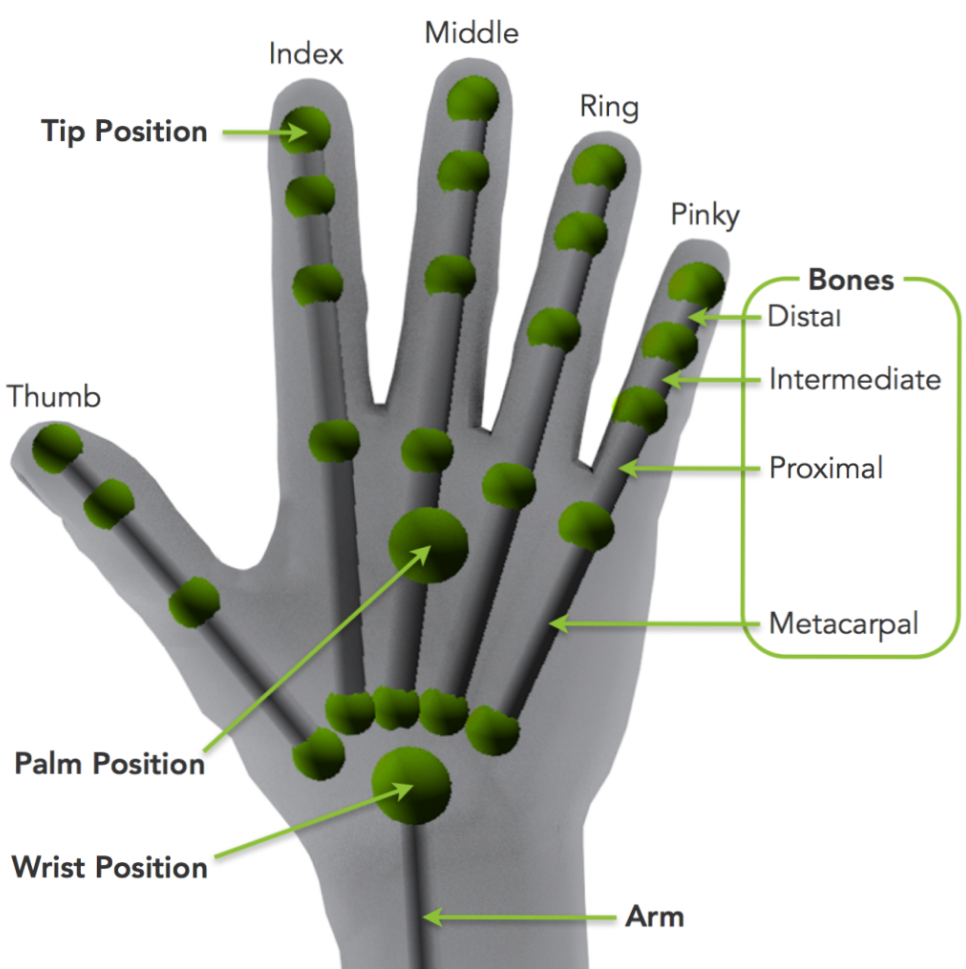
\includegraphics[scale=0.5]{Figures/handBones.png}
\caption[Hand Bone Model]{The Bones of the hand that Leap Motion device records data on. }
\label{fig:HandBones}
\end{figure}

A Hand object is only valid if it is detected by the Leap Motion device to be a physical object; if a Hand object is created via code using the Hand() constructor, that hand is considered “invalid” and will return true when the hand.invalid() method is called it. The information contained within a valid Hand object read in from the device is Read Only and can not be changed or updated. 

The Leap Motion device records numerical data about the hand and finger positions. Using the Hand class provided by the Leap Motion Java API and described above in the previous paragraph, a graphical model was constructed. For this GUI construction, a graphical representation of the hand was built using basic 3D geometric classes provided by the JavaFX framework. The bones of the hand model were represented by the Cylinder class and the joints were represented by the Sphere JavaFX class. This Hand model is contained inside the \verb UIHand_Simple Java class. This class extends a base abstract UIHand class which itself inherits from the JavaFX class called Group. Group is a type of Node in JavaFX that contains an ObservableList of children Nodes that will be added to the JavaFX Scene Graph in the order that they are added to the Group. An important point to note is that any transform, effect or property change applied to a Group will also be applied to all the children of that group. The figure below shows an example of how a Group Node can can contain multiple children nodes.

\begin{figure}[th]
\centering
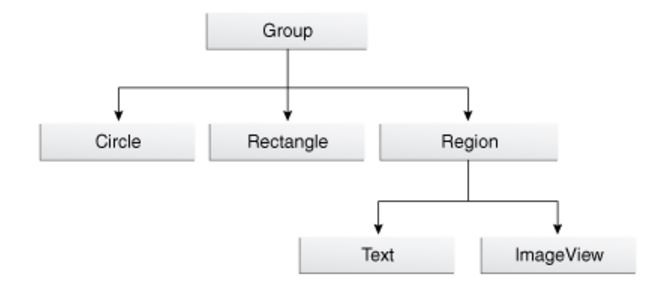
\includegraphics[scale=0.75]{Figures/javafx_group_node.JPG}
\caption[JavaFx Group Node]{The Group Node structure in the JavaFX framework. }
\label{fig:javafxGroupNode}
\end{figure}


The \verb UIHand_Simple class stores all the fingers bones in two dimensional array of Cylinder objects and all the respective joints in a different two dimensional array of Spheres. These arrays are of dimensions 5x3 to account for the five fingers and the three types of primary finger bones: distal, intermediate and proximal. In addition to these arrays, there is an array containing the four metacarpal bones of the hand; the thumb does not have a corresponding metacarpal bone like the other fingers. The also contains two more cylinders and a sphere to construct the palm section of the hand. To provide the hand with a uniform, well-blended color shading a PhongMaterial object is set as the hand’s material property. Figure \ref{fig:uihandsimpleConst} shows the initialization of the \verb UIHand_Simple and part of its constructor to illustrate how the hand model was designed.


\begin{figure}[th]
\centering
\begin{lstlisting}
public class UIHand_Simple extends UIHand {
    private static float fingerRadius = 14f;
	//Hand elements
    private Cylinder[][] fingerBones;
    private Sphere[][] fingerJoints;
    private Cylinder[] knuckleSpans;
	...
    public UIHand_Simple(Color color, boolean wireframe) {
        //Execute the Group constructor
        super();
        //Create the materials
        PhongMaterial dark = new PhongMaterial(color);
        PhongMaterial light = new PhongMaterial(color.brighter());
        //Initialize Finger bones
        fingerBones = new Cylinder[5][];
        for (int i = 0; i < 5; ++i) {
            fingerBones[i] = new Cylinder[3];
            for (int j = 0; j < 3; ++j) {
                fingerBones[i][j] = new Cylinder();
                //set material and radius and drawMode
                fingerBones[i][j].setMaterial(dark);
                fingerBones[i][j].setRadius(fingerRadius / ViewMath.radiusScaleFactor);
                if (wireframe) fingerBones[i][j].setDrawMode(DrawMode.LINE);
            }
		...
\end{lstlisting}
\caption[UIHandSimple Constructor]{A snippet of code showing how a the UIHandSimple class, representing the graphical hand, is constructed.}
\label{fig:uihandsimpleConst}
\end{figure}

Each element of the hand, such as all the cylinders and spheres representing the various bones and joints, is added to the children of the encompassing parent group that represents the hand.


%------------------------------------------------
%	SECTION 2 Set Location Method
%------------------------------------------------
\section{Set Location Method}
The \verb UIHand_Simple class also contains a method that allows for the graphical hand to be positioned according to the exact positions recorded in a Leap Motion Hand object. This method, which is called setLoc(Hand h), goes through each of the fingers and their respective bones and joints and sets the position and rotation of these these JavaFX nodes based upon the Hand object passed in. This method relies on a helper class called ViewMath which contains static methods that are called to position each individual cylinder representing a bone. Two of the important methods in ViewMath are setPositionByVector(Node n, Vector v) and setRotationByVector(Node n, Vector v). The method setPositionByVector sets the translate properties of the JavaFX Node passed in to the XYZ position recorded in the vector. The setRotationByVector method rotates the JavaFX Node passed into it by the direction which is represented by the second argument vector. This method first takes the direction and “corrects” it by flipping the z-value. This is done because JavaFX's coordinate system has the Z-axis increasing outward from the computer screen, while Leap Motion has the Z-axis increasing into the screen. The setRotationByVector finds the angle of rotation finding the the angle of the passed in direction to the Y-axis. In addition to the angle of rotation, the axis upon which the rotation will occur also needs to be defined. The axis of the rotation is found by taking the cross-product between the Y-axis and the “corrected” direction. Figure \ref{fig:setRotationByVectorCode} shows how rotation is set for nodes in the hand model.


\begin{figure}[th]
\centering
\begin{lstlisting}
//This method rotates a given JavaFx node to point in the direction passed in
public static void setRotationByVector(Node node, Vector direction) {
	//Correct the direction to correspond to JavaFx Coordinate system
	Vector correctedDirection = new Vector(direction.getX(), direction.getY(), -direction.getZ());
	//Find the angle of the direction to the y-axis; in degrees
	double angle = correctedDirection.angleTo(Vector.yAxis()) * 180 / Math.PI;
	//Find the axis of rotation by taking the cross product of the corrected direction with the y-axix
	Point3D axis = vectorToPoint(correctedDirection.cross(Vector.yAxis()));
	//Set the axis and angle of rotation on the Node object
	node.setRotate(angle);
	node.setRotationAxis(axis);
}
\end{lstlisting}
\caption[setRotationByVector Method]{A snippet of code showing how the rotation is set for an arbitrary Node object of the JavaFX Hand Model.}
\label{fig:setRotationByVectorCode}
\end{figure}




%------------------------------------------------
%	SECTION 3 Concurrency
%------------------------------------------------
\section{Concurrency}
One of the key concepts that is used in writing this project's application was that of concurrency. Concurrency in a JavaFX application is very important as it allows for the UI of to be responsive to user interactions despite the fact that the application might also be executeing other tasks in the background. In other to achieve this requirement, it is necessary to employ multithreading so that the main application thread can focus on responding to user interactions and other time-consuming tasks can be delegated to background threads. The UI in a JavaFX application is represented by the Scene Graph, which has been discussed earlier. The Scene Graph is not thread-safe and it should only be accessed and updated via the main running application thread, which is called the JavaFX Application thread. Implementing long running tasks on the JavaFX Application thread will invariably make the UI of the application unresponsive. The best practice to avoid this problem by letting the JavaFX Application thread focus on just processing user events. 


%----------------------------------- JavaFX Concurrent Package
\subsection{JavaFX Concurrent Package}
%
One might consider implementing the Runnable interface and creating their own thread objects from scratch to employ in the multithreaded environment required for building JavaFX applications. However, such an approach is not recommended; it can lead to unnecessary complexity and hard to debug problems such as deadlock, which is when competing threads are stuck waiting forever, and race conditions where critical data can be modified relatively simultaneously by two competing threads. 
(talk bout javafx concurrent package. lead into observable and util concurrency package. )


%----------------------------------- Project Application
\subsection{Project Application}
%













 (explain app can become unresponsive if we do things squetially. therefore we need to use the classes in javafx.concurrent package to achieve responsive and userfriendly experience.)



we are using javafx.concurrent package. read through docs and write notes about what to write and explain. 



In fact JavaFX is a framework that deals with concurrency to allow it to perform multiple tasks synchronously 





--read some code about javafx application threading stuff. research. 
write it in a paragraph and explain what it means. 

--look at the code that does task setting. read it a little try to understand. make some notes about what it means and how its wired. 
write about it. 

-- also write about the frame controller methods offered by leap ui. and talk about the controller2. read code, understand, make notes. and then write about it. 